%% 
%% Copyright 2007, 2008, 2009 Elsevier Ltd
%% 
%% This file is part of the 'Elsarticle Bundle'.
%% ---------------------------------------------
%% 
%% It may be distributed under the conditions of the LaTeX Project Public
%% License, either version 1.2 of this license or (at your option) any
%% later version.  The latest version of this license is in
%%    http://www.latex-project.org/lppl.txt
%% and version 1.2 or later is part of all distributions of LaTeX
%% version 1999/12/01 or later.
%% 
%% The list of all files belonging to the 'Elsarticle Bundle' is
%% given in the file `manifest.txt'.
%% 

%% Template article for Elsevier's document class `elsarticle'
%% with numbered style bibliographic references
%% SP 2008/03/01

\documentclass[preprint,12pt, a4paper]{elsarticle}



%% Use the option review to obtain double line spacing
%% \documentclass[authoryear,preprint,review,12pt]{elsarticle}

%% For including figures, graphicx.sty has been loaded in
%% elsarticle.cls. If you prefer to use the old commands
%% please give \usepackage{epsfig}

%% The amssymb package provides various useful mathematical symbols
\usepackage{amssymb}
\usepackage{hyperref}
\setlength{\parindent}{0pt}
%% The amsthm package provides extended theorem environments
%% \usepackage{amsthm}

%% The lineno packages adds line numbers. Start line numbering with
%% \begin{linenumbers}, end it with \end{linenumbers}. Or switch it on
%% for the whole article with \linenumbers.
%\usepackage{lineno}

\journal{SoftwareX}

\begin{document}
\renewcommand{\labelenumii}{\arabic{enumi}.\arabic{enumii}}

\begin{frontmatter}

 
%% Title, authors and addresses

%% use the tnoteref command within \title for footnotes;
%% use the tnotetext command for theassociated footnote;
%% use the fnref command within \author or \address for footnotes;
%% use the fntext command for theassociated footnote;
%% use the corref command within \author for corresponding author footnotes;
%% use the cortext command for theassociated footnote;
%% use the ead command for the email address,
%% and the form \ead[url] for the home page:
%% \title{Title\tnoteref{label1}}
%% \tnotetext[label1]{}
%% \author{Name\corref{cor1}\fnref{label2}}
%% \ead{email address}
%% \ead[url]{home page}
%% \fntext[label2]{}
%% \cortext[cor1]{}
%% \address{Address\fnref{label3}}
%% \fntext[label3]{}

\title{quicR: An R Library for Streamlined Data Handling of Real-Time Quaking Induced Conversion Assays}

\author[label1,label2,label3]{Gage Rowden\corref{cor}\fnref{email}}
\ead{rowde002@umn.edu}
\fntext[email]{}
\cortext[cor]{}
\author[label1,label2,label3]{Peter Larsen}
\address[label1]{Department of Veterinary and Biomedical Sciences, University of Minnesota, St. Paul, MN 55108, USA.}
\address[label2]{Minnesota Center for Prion Research and Outreach, University of Minnesota, St. Paul, MN 55108, USA.}
\address[label3]{Priogen Corp., St. Paul, MN 55114, USA.}

\begin{abstract}
Real-time quaking induced conversion (RT-QuIC) has quickly become a valuable diagnostic tool for protein misfolding disorders such as Creutzfeldt-Jakob disease and Parkinson's disease. Given that the technology is relatively new, academic and industry standards for quality filtering data and high throughput analysis of results have yet to be fully established. The open source R library, quicR, was developed to provide a standardized approach to RT-QuIC data analysis. quicR provides functions, which can be easily integrated into existing R workflows, for data curation, analysis, and vizualization.
\end{abstract}

\begin{keyword}
%% keywords here, in the form: keyword \sep keyword
R package \sep RT-QuIC \sep prion \sep diagnostics \sep CJD \sep Parkinson's

%% PACS codes here, in the form: \PACS code \sep code

%% MSC codes here, in the form: \MSC code \sep code
%% or \MSC[2008] code \sep code (2000 is the default)

\end{keyword}

\end{frontmatter}

% \linenumbers

\section*{Metadata}
\label{}
\textit{The ancillary data table~\ref{codeMetadata} is required for the sub-version of the codebase. Please replace the italicized text in the right column with the correct information about your current code and leave the left column untouched.}

\begin{table}[ht]
\begin{tabular}{|l|p{6.5cm}|p{6.5cm}|}
\hline
\textbf{Nr.} & \textbf{Code metadata description} & \textbf{Metadata} \\
\hline
C1 & Current code version & V2.1.0 \\
\hline
C2 & Permanent link to code/repository used for this code version & \url{https://github.com/gage1145/quicR} \\
\hline
C3  & Permanent link to Reproducible Capsule & \url{https://github.com/gage1145/quicR/releases/tag/v2.1.0}\\
\hline
C4 & Legal Code License   & GPL-3 \\
\hline
C5 & Code versioning system used & git \\
\hline
C6 & Software code languages, tools, and services used & R \\
\hline
C7 & Compilation requirements, operating environments \& dependencies & R (>=4.1.0) \\
\hline
C8 & If available Link to developer documentation/manual & \url{https://cran.r-project.org/web/packages/quicR/quicR.pdf} \\
\hline
C9 & Support email for questions & rowde002@umn.edu\\
\hline
\end{tabular}
\caption{Code metadata}
\label{codeMetadata} 
\end{table}


\section{Motivation and significance}
    Real-time quaking induced conversion (RT-QuIC) is a cutting-edge diagnostic assay that has garnered significant attention for its ultra-sensitive detection of misfolded protein aggregates \cite{Wilham2010, Atarashi2011}. The assay works by converting a recombinant protein substrate into an amyloid aggregate in the presence of a misfolded seed \cite{Wilham2010, Orru2012, Orru2017, Orru2015, Bongianni2019, Dassanayake2016, Hwang2018, Groveman2018, Metrick2020}. The assay's sensitivity and specificity make RT-QuIC a promising tool for diagnosing diseases such as prion disorders and other protein misfolding pathologies \cite{Fiorini2020, Franceschini2017, Picasso-Risso2022, Holz2021}. However, the relatively recent development and novelty of the assay have left a gap in widely accepted academic and industry standards for data analysis and interpretation \cite{Rowden2023}.

    To address this gap, we introduce quicR, an open-source library, developed in R \cite{R2024}, dedicated to the cleaning, analysis, and visualization of RT-QuIC data. By consolidating key metrics and providing robust analytical tools, quicR aims to standardize the analysis pipeline and foster reproducibility within the field of quaking induced assays including related assays such as Nano-QuIC \cite{Christenson2023} and Micro-QuIC \cite{Lee2024}. quicR is designed with both researchers and diagnosticians in mind, providing a user-friendly interface that integrates seamlessly with existing R workflows.

    While universal diagnostic criteria for RT-QuIC have yet to be established, certain analytical metrics have emerged as valuable tools for interpreting assay results and kinetics. These include:

    \begin{enumerate}
        \item Time-to-threshold (TtT): The time required for the fluorescence signal to exceed a predefined threshold \cite{Orru2015}.
        \item Rate of amyloid formation (RAF): A measure of the kinetics of aggregate growth, which provides insight into the relative quantity of misfolded seed \cite{Gallups2022}.
        \item Maxpoint ratio (MPR): A ratio-based metric measuring peak normalized fluorescence intensities \cite{Rowden2023}.
        \item Maximum slope (MS): The steepest rate of fluorescence increase, reflecting the most rapid phase of aggregation \cite{Henderson2015}.
    \end{enumerate}

    Together, these metrics enable researchers to characterize the kinetics of RT-QuIC reactions comprehensively, enhancing the rigor and reliability of diagnostic decisions.

    In addition to analytical tools, quicR provides flexible and customizable visualization capabilities. Leveraging the powerful ggplot2 library \cite{ggplot2016}, quicR enables users to generate high-quality, publication-ready figures. These visualizations can be further customized using the intuitive '+' syntax of ggplot2, allowing for tailored presentations of RT-QuIC data.

    By combining standardized metrics, advanced visualization tools, and a commitment to open source science, quicR serves as a foundational resource for the growing RT-QuIC community. Its goal is to empower researchers to analyze and present their data with clarity, consistency, and cohesion.

\textit{In this section, we want you to introduce the scientific background and the motivation for developing the software.}

\begin{itemize}
    \item \textit{Explain why the software is important and describe the exact (scientific) problem(s) it solves.}
    \item \textit{Indicate in what way the software has contributed (or will contribute in the future) to the process of scientific discovery; if available, please cite a research paper using the software.}
    \item \textit{Provide a description of the experimental setting. (How does the user use the software?)}
    \item \textit{Introduce related work in literature (cite or list algorithms used, other software etc.).}
\end{itemize}

\section{Software description}
    \subsection{Software architecture}
        quicR was developed to address the growing need for efficient data conversion, analysis, and visualization of RT-QuIC data. With a focus on usability and reproducibility, the package is designed to standardize workflows and ensure compatibility across multiple laboratories. Its primary input format is data exported as Excel workbooks from the proprietary MARS software (BMG Labtech, Ortenberg, Germany), providing seamless integration with existing experimental workflows. See Figure \ref{fig:workflow} for a detailed workflow.
        \begin{figure}[ht]
            \caption{Workflow hierarchy of the quicR package. Blue nodes indicate steps where BMG software is needed. Purple nodes indicate functions dedicated to handling metadata. Red nodes are functions that acquire and manipulate raw data. Orange nodes are functions which calculate some metric. Finally, yellow nodes represent data analysis endpoints.}
            \centering
            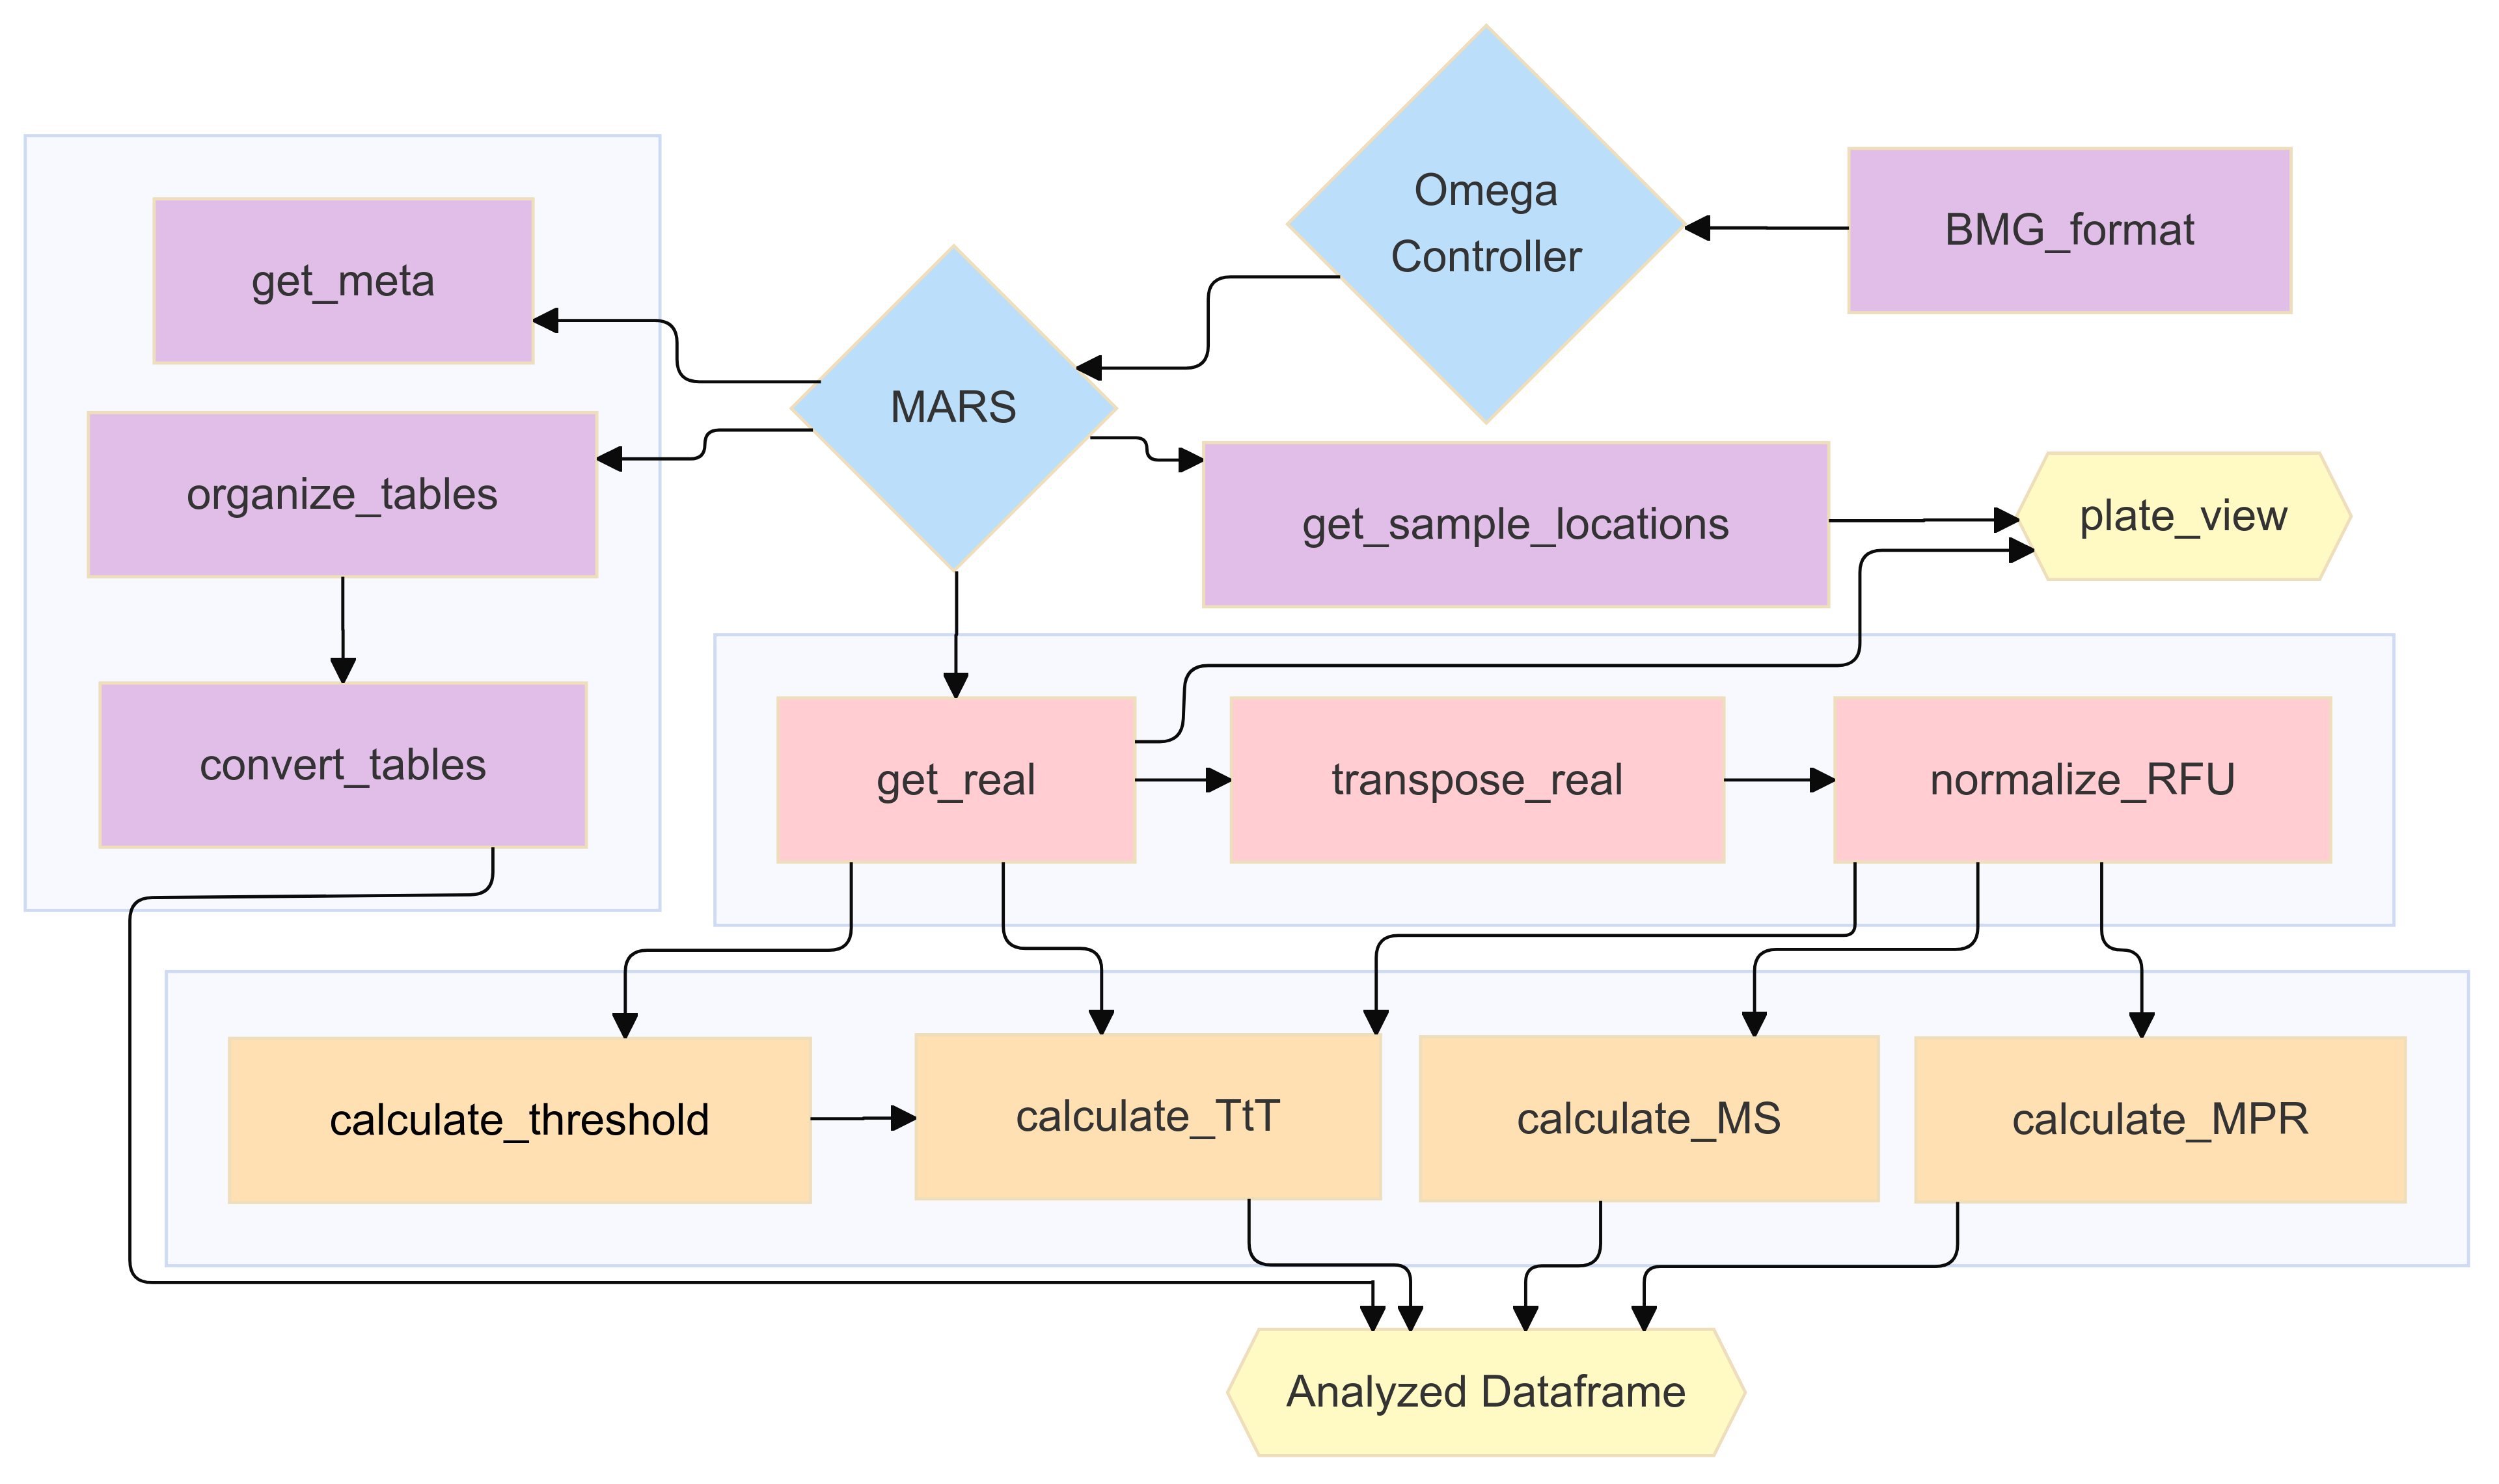
\includegraphics[width=\textwidth]{images/workflow2.png}
            \label{fig:workflow}
        \end{figure}

\subsection{Software functionalities}
\textit{  Present the major functionalities of the software.}
  
 \subsection{Sample code snippets analysis (optional)}


\section{Illustrative examples}

% \textit{Provide at least one illustrative example to demonstrate the major
% functions of your software/code.}

% \textit{\textbf{Optional}: you may include one explanatory  video or screencast that will appear next to your article, in the right hand side panel. Please upload any video as a single supplementary file with your article. Only one MP4 formatted, with 150MB maximum size, video is possible per article. Recommended video dimensions are 640 x 480 at a maximum of 30 frames / second. Prior to submission please test and validate your .mp4 file at  \url{http://elsevier-apps.sciverse.com/GadgetVideoPodcastPlayerWeb/verification} . This tool will display your video exactly in the same way as it will appear on ScienceDirect. }

\section{Impact}
\textit{This is the main section of the article and reviewers will weight it appropriately.
Please indicate:}
\begin{itemize}
    \item \textit{Any new research questions that can be pursued as a result of your software.}
    \item \textit{In what way, and to what extent, your software improves the pursuit of existing research questions.}
    \item \textit{Any ways in which your software has changed the daily practice of its users.}
    \item \textit{How widespread the use of the software is within and outside the intended user group (downloads, number of users if your software is a service, citable publications, etc.).}
    \item \textit{How the software is being used in commercial settings and/or how it has led to the creation of spin-off companies.}
    \end{itemize}
% \textit{Please note that points 1 and 2 are best demonstrated by
%   references to citable publications.}

\section{Conclusions}
    quicR offers a powerful solution for the cleaning, analysis, and visualization of RT-QuIC data, addressing critical needs in a rapidly evolving field. By enabling consistent data handling and interpretation, quicR lays the groundwork for improved diagnostic consistency and reproducibility. The package's open-source nature ensures that it will continue to evolve, integrating new insights and technologies as they emerge.

    As RT-QuIC technology advances, tools like quicR will play a pivotal role in bridging the gap between assay development and practical application. By equipping researchers with reliable, standardized tools, quicR not only supports the study of prion and protein misfolding disorders but also serves as a model for the development of software solutions in other diagnostic fields.

\section*{Acknowledgements}
\label{}
Special thanks to Beni Altmann at The Comprehensive R Archive Network (CRAN) for help during the submission process to CRAN. We thank Tiffany Wolf and Marc Schwabenlander for their support through the Minnesota Center for Prion Research and Outreach. We would like to acknowledge Suzanne Stone and Sarah Gresch for maintaining lab operations.


%% The Appendices part is started with the command \appendix;
%% appendix sections are then done as normal sections
%% \appendix

%% \section{}
%% \label{}

%% References:
%% If you have bibdatabase file and want bibtex to generate the
%% bibitems, please use
%%
\bibliographystyle{elsarticle-num} 
\bibliography{references.bib}

% \textit{If the software repository you used supplied a DOI or another
% Persistent IDentifier (PID), please add a reference for your software
% here. For more guidance on software citation, please see our guide for
% authors or \href{https://f1000research.com/articles/9-1257/v2}{this
%   article on the essentials of software citation by FORCE 11}, of
% which Elsevier is a member.}

% \large{\textbf{Reminder: Before you submit, please delete all 
% the instructions in this document, 
% including this paragraph. 
% Thank you!}}





\end{document}
\endinput
%%
%% End of file `SoftwareX_article_template.tex'.

%%% Local Variables:
%%% mode: latex
%%% TeX-master: t
%%% End:
